\section{Theory}\label{sec:Theory}

\subsection{The Ising Model}\label{subsec:ising}

The Ising model is a model for describing binary lattice systems. When cast in
the language of physics, the values are regarded as spin, with properties such
as energy, magnetization and phase transition being investigated. The phase
transition only occur in two or more dimensions. Its analytical description
solution was found by Lars Onsager in 1944~\cite{onsager}. 

For the one dimensional model the energy is described by

\begin{equation*}
  E[s^{i}] = -J\sum_{j=1}^{N}s_{j}s_{j+1}
\end{equation*}

with \(J\) as the coupling constant and \(s^{i}\) as a given spin state. The boundaries are periodic.

By lifting the constraint of only summing over nearest neighbors, the model can
be recast to a linear regression problem. The energy is now

\begin{align*}
  E[s^{i}] &= -\sum_{j,k=1}^{N}J_{j,k}s_{j}^{i}s_{k}^{i}\\
  &= \vb{X}^{i}\cdot\vb{J}\numberthis\label{eq:1}
\end{align*}

with \(\vb{X}^{i}\) the vector over two body interactions and \(\vb{J}\) the
coupling coefficients. The regression can then be performed on the set
\(\{E[s^i], s^{i}\}\).

When moving on to two dimensions, the Ising model exhibits phase transitions.
Under the critical temperature \(T_{C}/J \approx 2.27\) the system is in an
ordered phase with (almost) all spins pointing in the same direction. Above this
temperature the system is in an disordered phase with spins randomly oriented.
Examples of this are shown in~\cref{fig:matrix}. For practical purposes, ordered
phases have \(T/J<2.0\) and disordered \(T/J > 2.5\).

\begin{figure}
  \centering
  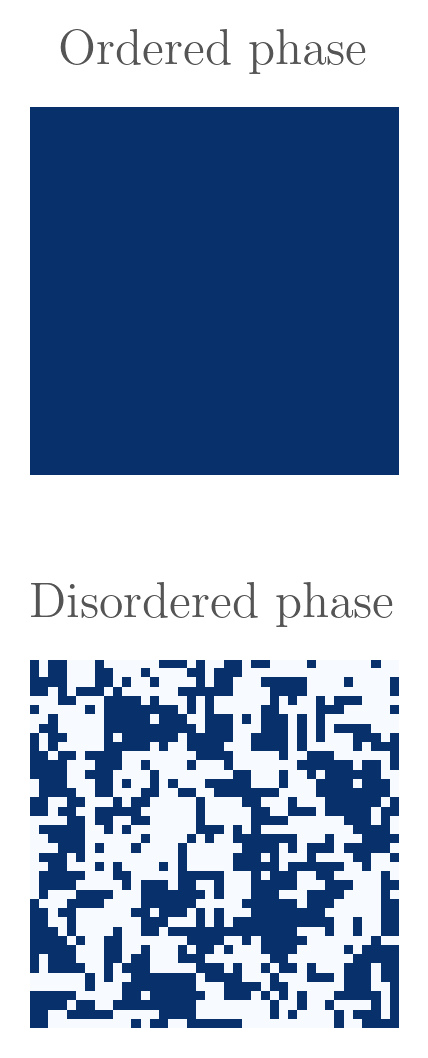
\includegraphics[]{figures/matrix.png}
  \caption{\label{fig:matrix} Examples of ordered and disordered phase systems
    used in classification.}
\end{figure}

\subsection{Logistic Regression}

In order to classify systems as either ordered or disordered, logistic
regression is performed. Classification problems with linear regression methods have data which is assigned to
one of \(K\) classes using an indicator response variable \(\hat f_{k}= \hat
\beta_{k0} + \hat\beta_{k}^{T}x\). 

Our case is binary with \(K=2\), hence \(y_{i} \in \{0,
1\} = \{ordered, disordered\}\). A popular choice is the sigmoid function,
giving

\begin{align*}
  p(y_{i} = 0 | x_{i},\hat\beta)  &= \frac{\exp(\hat{\beta}_{0} + 
                                    \hat\beta_{1}x_{i})}{1 + \exp(\hat\beta_{0} + \hat\beta_{1}x_{i})}\\
  p(y_{i} = 1 | x_{i},\hat\beta) &= 1 - p(y_i = 0 | x_{i},\hat\beta)
\end{align*}

By minimizing the likelihood we obtain the loss function \textit{cross entropy}~\cite{statelem}

\begin{align*}
  \mathcal{C}(\hat\beta) = \sum_{i=1}^{n}\left( y_{i}\log{p(y_{i}=1|x_{i},\hat\beta)} +
  (1-y_{i})\log{\left[ 1-p(y_{i}=1|x_{i},\hat\beta) \right]}\right)
\end{align*}

Classifying binary data is then equivalent to minimizing the cross entropy
function. This is achieved using gradient descent.

\subsection{Gradient Descent}

Gradient descent is a group of methods to minimize some parameters \(\theta\)
under a function \(f\).
The decrease is fastest in the direction of the gradient \(-\nabla f(\theta)\). By
iteration we then get

\begin{align*}
  \theta_{i+1} = \theta_{i} - \eta\nabla f(\theta_{i})
\end{align*}

where \(\eta\) is the step-size or \textit{learning rate}.

The method has a tendency to slow down when approaching a minima and the
gradient gets small. One way to remedy this is to add \textit{momentum}, giving

\begin{align*}
  v_{i} &= \mu v_{i-1} + \eta\nabla f(\theta_{i})\\
  \theta_{i+1} &= \theta_{i} - v_{i}
\end{align*}

with \(\mu\) the momentum hyperparameter.

Another benefit is that momentum makes the method more resilient to oscillations.

More can be gained by taking advantage of the fact that the gradient gives more
information about a minima the closer it is. By computing the gradient at the
\textit{expected} value given the current momentum, we obtain \textit{Nesterov
  accelerated gradient}:
\begin{align*}
  v_{i} &= \mu v_{i-1} + \eta\nabla f(\theta_{i} + \eta v_{i-1})\\
  \theta_{i+1} &= \theta_{i} - v_{i}
\end{align*}

This gives faster convergence for a given learning rate.

\subsection{Neural Networks}\label{subsec:neuralnet}

Neural networks is a machine learning algorithm inspired by biological neurons,
and has achieved impressive performance on a wide class of problems. A neuron is
modeled by a \textit{perceptron}, with perceptrons stacked together in layers
and layers stacked together into a network architecture. The first layer takes
an input vector \(\vb{x}\) of \(d\) features and produces an \textit{activation}
\(a_{i}(\vb{x})\). The activation is feed into the next layer, called
\textit{hidden layer}, and so on until
the last layer, the \textit{output layer}.

A layer transforms its input but first applying an
affine transformation on the form

\begin{align*}
  z^{(i)} = \vb{W}^{(i)}\vb{x} + b^{i}
\end{align*}

with \(\vb{W^{i}}\) being the \textit{weights} of layer \(i\) and \(b^{i}\) its
bias. This is followed by a non-linear transformation

\begin{align*}
  a_{i}(\vb{x}) = \sigma_{i}(z^{(i)})
\end{align*}
The \textit{activation function } \(\sigma_{i}\) is specific to each layer. 
The activation function of the output layer determines whether the network is a
classifier, in which the function is a sigmoid or softmax function, or linear,
where the function is linear.

This combination of linear and non-linear transformations allows a network to
approximate any function to arbitrary precision, a result known as the universal
approximation theorem\cite{mehta}. In order to achieve this expressive power,
the network has to be trained. This is done by an algorithm known as
\textit{backpropagation}.

\subsubsection{Backpropagation}

To train a network, a cost function is optimized. For linear regression this is
often the mean square error, while for classification this is often the cross
entropy. The optimization is done by gradient descent, where an input is feed
forward through the network, compared to the expected output, and the error is
fed backwards and used to update the weights and biases. This backpropagation of
the error is essentially the chain rule from calculus applied recursively.

The four equations of backpropagation are

\begin{align*}
  \delta_{j}^{l} &= \pdv{E}{a_{j}^{l}}\sigma\prime\left( z_{j}^{l} \right)\\
  \delta_{j}^{l} &= \pdv{E}{b_{j}^{l}}\\
  \delta_{j}^{l} &= \left( \sum_{k}\delta_{k}^{l+1}w_{kj}^{l+1} \right)\sigma\prime\left( z_{j}^{l} \right)\\
  \pdv{E}{w_{jk}^{l}} &= \delta_{j}^{l}a_{k}^{l-1}
\end{align*}

A deeper explanation of these equation and their derivation can be found in
literature, such as~\cite{mehta}.


\subsection{Activation Functions}

There are a wide arrange of activation functions available, with new ones
proposed and their virtues hailed in papers. Here three common activation
functions will be studied: the sigmoid, the rectified linear unit (ReLU) and
leaky ReLU. These are plotted in~\cref{fig:activations}.

All are non-linear, as is required for a network to learn; if a network only had
a linear transformation, the entire network would be nothing more than linear
transformation. The functions are similar in their behavior, with some important
differences. The sigmoid suffers from \textit{vanishing derivative}, where the
gradient can be vanishingly small and prevent weights from updating. The ReLU
rectify this problem as it only saturates in one direction, and the leaky ReLU
doesn't have any saturation, and does not suffer from this problem. In addition,
ReLU and leaky ReLU have been found to outperform the sigmoid, giving faster learning.\cite{mehta}\cite{statelem}.

\begin{figure*}[]
  \centering
  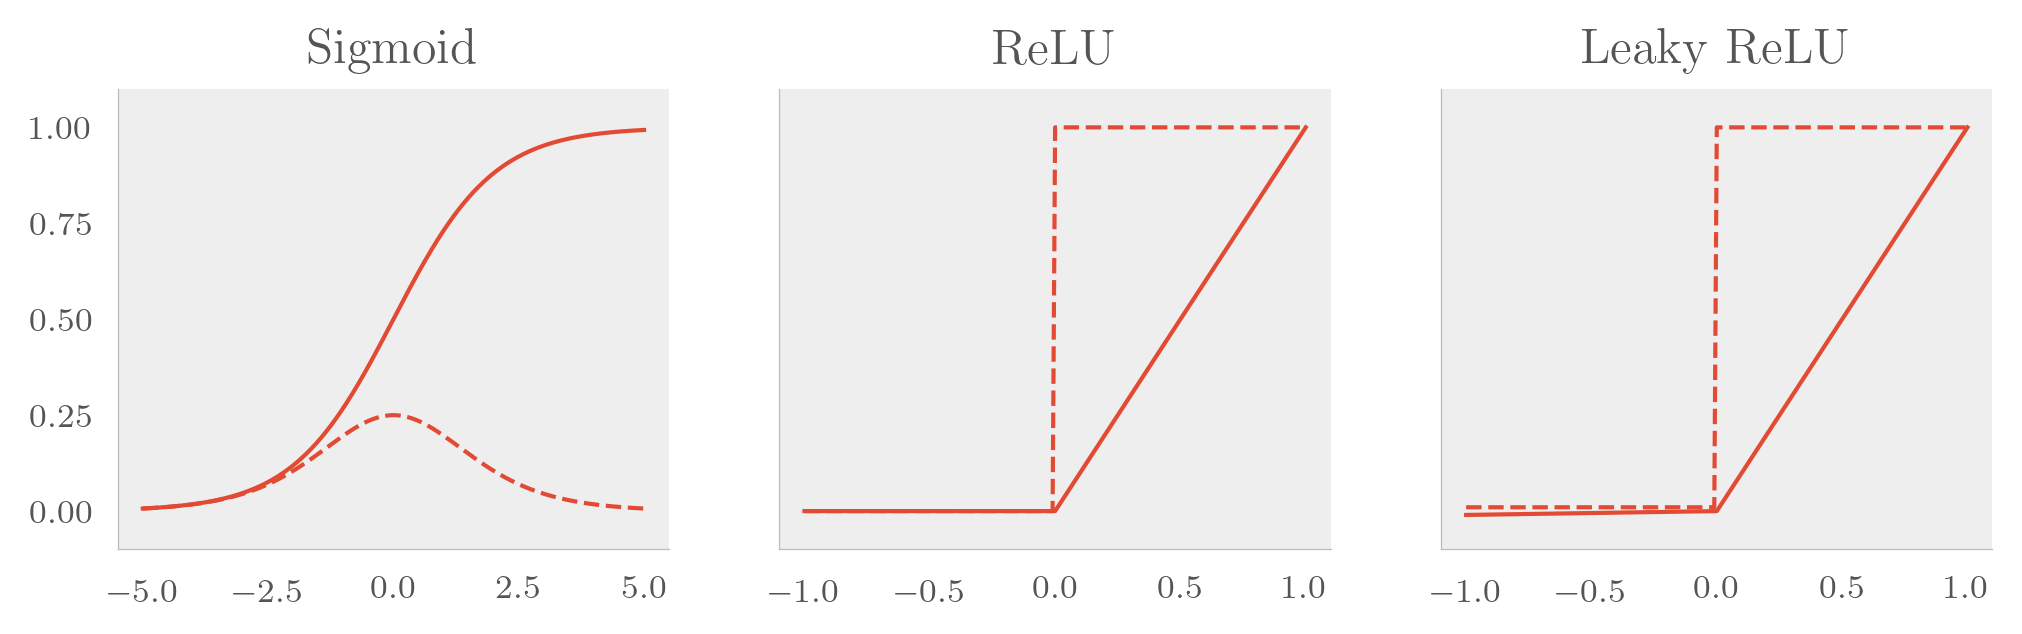
\includegraphics[]{figures/activations.png}
  \caption{\label{fig:activations} The three activation functions studied. The
    whole lines show the functions themselves while the dashed their
    derivatives. The sigmoid has vanishing derivatives at both ends, ReLU at the
  negative side, while the leaky ReLU does not have any vanishing derivatives.
  The two latter lack continuous derivatives, seen by the jump at 0.}
\end{figure*}

